Some parts of this question expect you to extract information from a  set of tables reproduced from the latest edition of `The Review of Particle Physics'.
These tables (which can be found after the statement of the question) may include both: (i) information which is irrelevant to you, and (ii) terms or symbols which are not fully explained.  The question is therefore testing your ability to extract information from unfamiliar  sources regularly used in particle physics research.
\begin{allparts}
\part
Explain why the positively charged pion's decay mode to $\mu^+\nu_\mu$ dominates over its decay to $e^+\nu_e$.\marks{3}

\ANS{

BOOKWORK: description of parity violation, ang mom conservation, scalar nature of pion, neutrinos all left handed, etc.

}
\part
Looking at the decay modes of the $\pi^0$, suggest possible reasons for the difference between the branching fractions stated for the $e^+e^+e^-e^-$ and  $e^+e^-$ final states.\marks{4}

\ANS{

This is a tough question as the (strong) preference for the four-electron final state over the two-electron final state will be DOUBLY counter-intuitive to the students who have been brought up (1) vertex counting, and (2) looking at phase space.  [There are more vertices in the Feynman diagram for $\pi^0\rightarrow e^+e^+e^-e^-$  than for $\pi^0\rightarrow e^+e^+$, and the final state with four electrons is heavier than that with two!]  I am not looking for any specific or correct answer to this question [hence `suggest' rather than `state'/`explain']. Rather I am looking to see candidate making sensible statements which make clear that they are mentally processing (or even can see) the challenge faced by the discrepancy seen here.     E.g.,~there could be some marks for a candidate observing that the preference goes against a `simple' analysis for the two reasons already mentioned and so must be related to some other constraints/principles.  It is conceivable that some candidates will look at the decay table and note that $\pi^0\rightarrow \gamma\gamma$  dominates over all other decay modes by a long way. Though they may not know that this is due to $C$-parity ($C$-parity is not in the Part-II course lectures, but does come up in passing in Prob Sheet 2, Q13a) they may at least report that WHATEVER it is that leads to the favouring of $\gamma\gamma$ final states could lead to bleed-through into $\gamma e^+e^-$ and from there into $ e^+e^+e^-e^-$ as a result of off-shell photons going to $e^+e^-$. They might even note that this would account for the approximately equal spacing (in log space) of the branching ratios for those three modes. Perhaps candidates will have ideas that are very different from those I've suggested here. So long as they are intelligent statements derived from things they were learning about in the course, and are accurately applied, they will be rewarded, even if they don't ultimately explain the preference for four electrons. 

}
\part
Draw the lowest order Feynman diagrams for the processes   (i) $\pi^0 \rightarrow \pi^+ e^- \bar \nu_e$ and (ii) $\pi^+ \rightarrow e^+ \nu_e \pi^0$.  Why do the tables list a branching ratio for only one of these two processes?  What branching ratio is reported for it?  What physical reasons might lead to it being that big or that small?\marks{5}

\ANS{

50\% of the marks are for just drawing valid Feynman diagrams containing a single $W$ connected to the right things (with no gluons or photons hanging around).  
Then they need to point out that the mass of the $\pi^+$ is bigger than that of the $\pi^0$ and so the $\pi^0$ cannot have decays involving $\pi^+$ on kinematic grounds.  The branching ratio for $\pi^+ \rightarrow e^+ \nu_e \pi^0$ is very small ($1.03\times 10^{-8}$).  An important point affecting the smallness of this branching ratio is that the $\pi^+$ and $\pi^-$ mass difference is itself very very small (only 4.5 MeV, relative to 140 MeV for the mass of the $\pi^+$ itself).  This means that there is already a factor of 30 (i.e.~140/4.5) more phase space for decays without a pion in the final state than for those with one. On top of that, there are extra vertices to throw into the calculation to generate the pion. 

}
\part
%Why is no decay mode table given for the $\pi^-$ ? 
Make a prediction for the $\pi^-$ branching fraction into (i) $\mu^-\bar\nu_\mu \gamma$ and (ii) $e^-\nu_e e^- e^+$.\marks{2}

\ANS{

%The $\pi^-$ decay modes table is not given as decay modes can be inferred from the supplied $\pi^+$ table after $CP$-conjugating each row.  [1 mark] This is valid ias $CP$-violation is not important for pions. [1 marks]

Part (i) here is almost a dummy question whose purpose is not to check the answer ($(2.00\pm0.25)\times 10^{-4}$) but to make it clear that the question setter will put bars on neutrinos when required.  It is necessary to flag that willingness up here so that the part (ii) can be validly asked/answered. [1 mark off if wrong, though]

The answer to part (ii) is \textbf{zero} because the CP conjugation of 
$e^-\nu_e e^- e^+$ is $e^+\bar\nu_e e^+ e^-$ and there is no such line in the PDG's $\pi+$ decay table. The table only has a line for $e^+\nu_e e^+ e^-$.  The suggested mode violates lepton number. [2 marks total. One for saying the BR is zero,  and one for explaining why.]

}

\part
Suppose that a $\Xi^0$ baryon is produced in a vacuum at the centre of an infinitely large box at time $t_0=0$. 
What are the most probable contents of the box if inspected at a later time $t_1=10^{-12}$~s?  Describe the two main routes or `histories' through which the contents of the box might be expected to evolve over time.  Cover the period from $t_0$ until the contents of the box reach steady state, making clear on what timescales different events might be expected to happen.  How probable are the two end states you have considered? \marks{5}

\ANS{

This question asks the candidates to look at all the decay tables and plot a route through for the decay of the $\Xi^0$.  They should see the following:
\begin{itemize}
\item
The lifetime of the $\Xi^0$ is $\tau_\Xi=2.9\times 10^{-10}$~s, so very little can be expected to have happened on time scales much shorter than that.
\item
That by/around  $\tau_\Xi$ the $\Xi^0$ stands a good chance of having decayed, and if it has decayed, the vast majority of decays are to $\Lambda \pi^0$.
\item
However, the lifetime of the $\pi^0$ is $\tau_{\pi_0}=8\times 10^{-17}$~s which is much shorter than $\tau_\Xi$. Therefore, when the $\Xi$ decay eventually takes place it will (for all practical purposes) look like a decay to $\Lambda \gamma \gamma$ -- one has only a vanishing chance of being there at the right time to see both a $\Lambda$ and a not-yet-decayed $\pi_0$.
\item
The $\Lambda$ has a similar lifetime to the $\Xi$, so on a similar timescale to the $\Lambda$ being created it is likely to be replaced (with probability $\sim64$\%) by $p\pi^-$ or (with probability $\sim35$\%) by a $n\pi^0$ which will `instantly' become $n\gamma\gamma$.
\item
The lifetime of the $\pi^-$ is, however, longer than those we've seen before, $\tau_{\pi^-}=10^{-8}$~s (on account of helicity suppression) so the disappearance of the $\pi^-$ will take place over a time of order $\tau_{\pi^-}$.
\item By around $t=10^{-7}$~s all the $\pi^+$ will have died away and so we will either find the box containing $p\mu\bar\nu_\mu\gamma\gamma$ (with probability $\sim64$\%) or $n\gamma\gamma\gamma\gamma$ (with probability $\sim35$\%).
\item
Things will stay much like that until the neutrons begin to decay, which should be complete when $t\gg 880$~s (the lifetime of the neutron).
\item
The final state is therefore $p\mu\bar\nu_\mu\gamma\gamma$ (with probability $\sim64$\%) or $p e^-\bar\nu_e\gamma\gamma\gamma\gamma$ (with probability $\sim35$\%).
\end{itemize}
One could award about half a mark per bullet point above.
}
\end{allparts}

%\begin{allparts}
%\end{allparts}

%\begin{allparts}
%\end{allparts}

%\begin{allparts}
%\end{allparts}

%\begin{allparts}
%\end{allparts}

%\begin{allparts}
%\end{allparts}

%\begin{allparts}
%\end{allparts}

%\begin{allparts}
%\end{allparts}

%\begin{allparts}
%\end{allparts}

\begin{center}
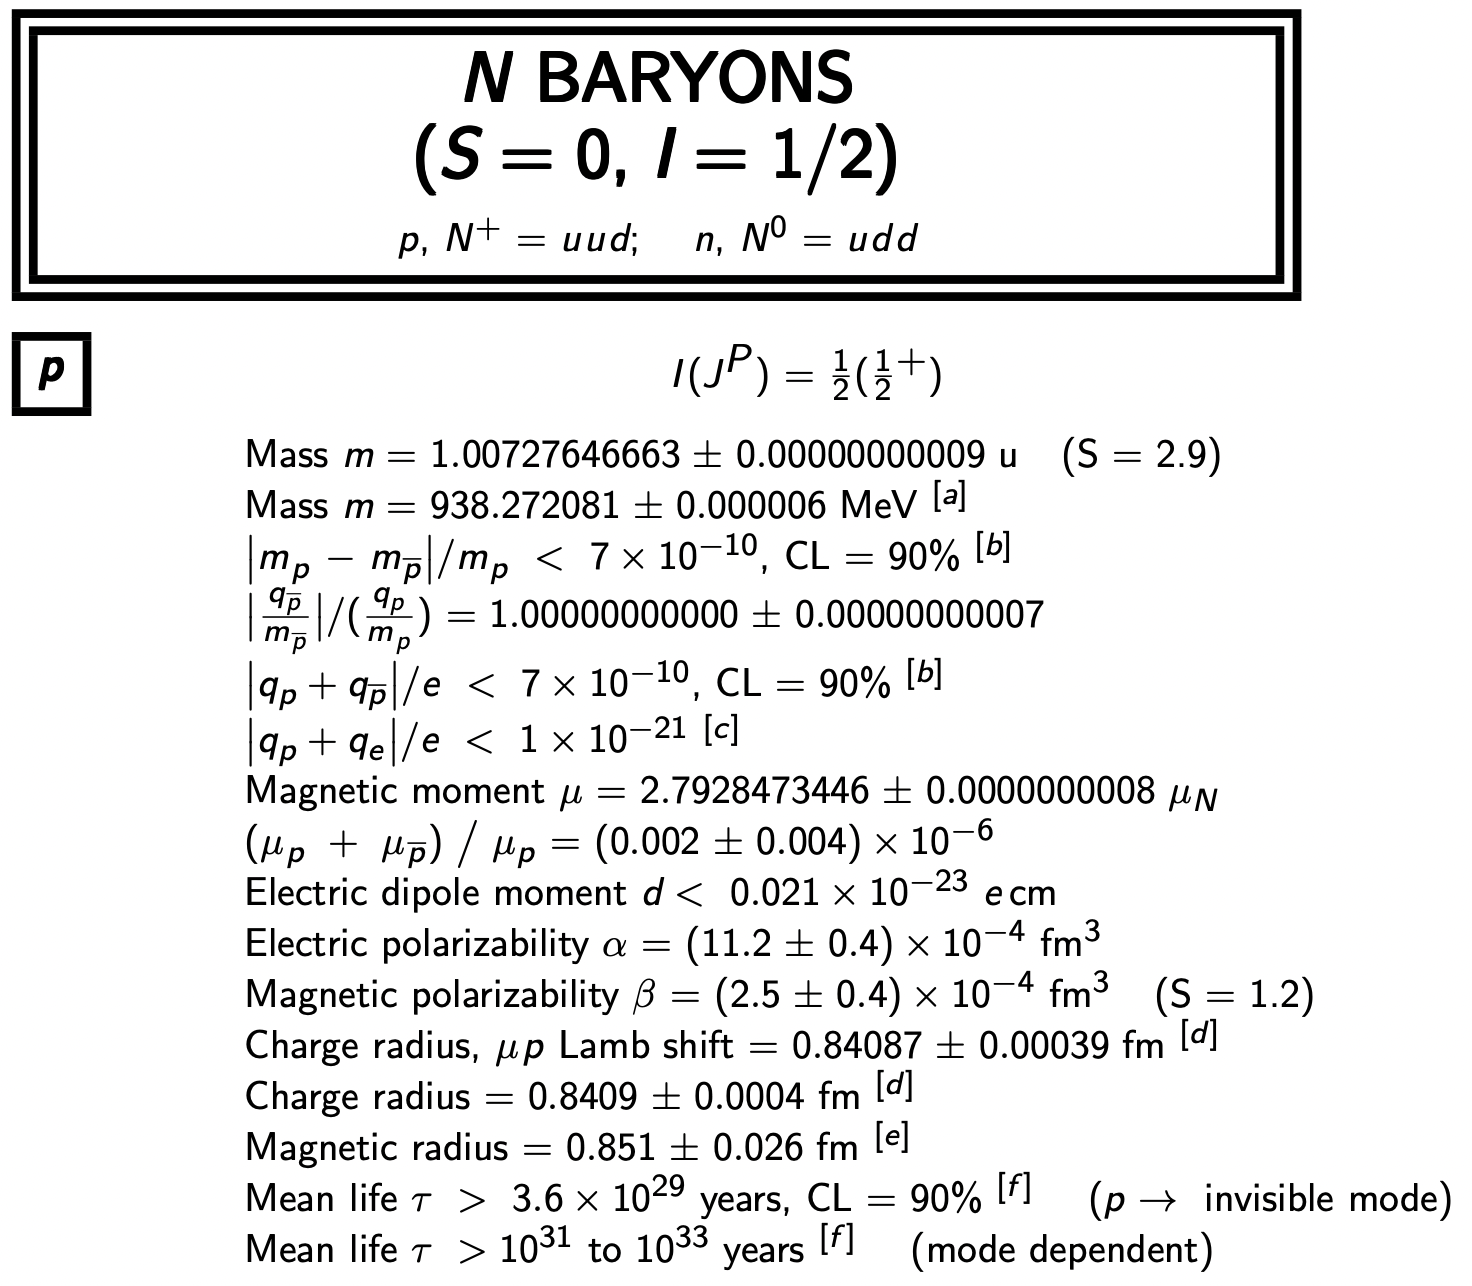
\includegraphics[width=0.8\textwidth]{PDG/N_BARYONS_AND_PROTON.png}
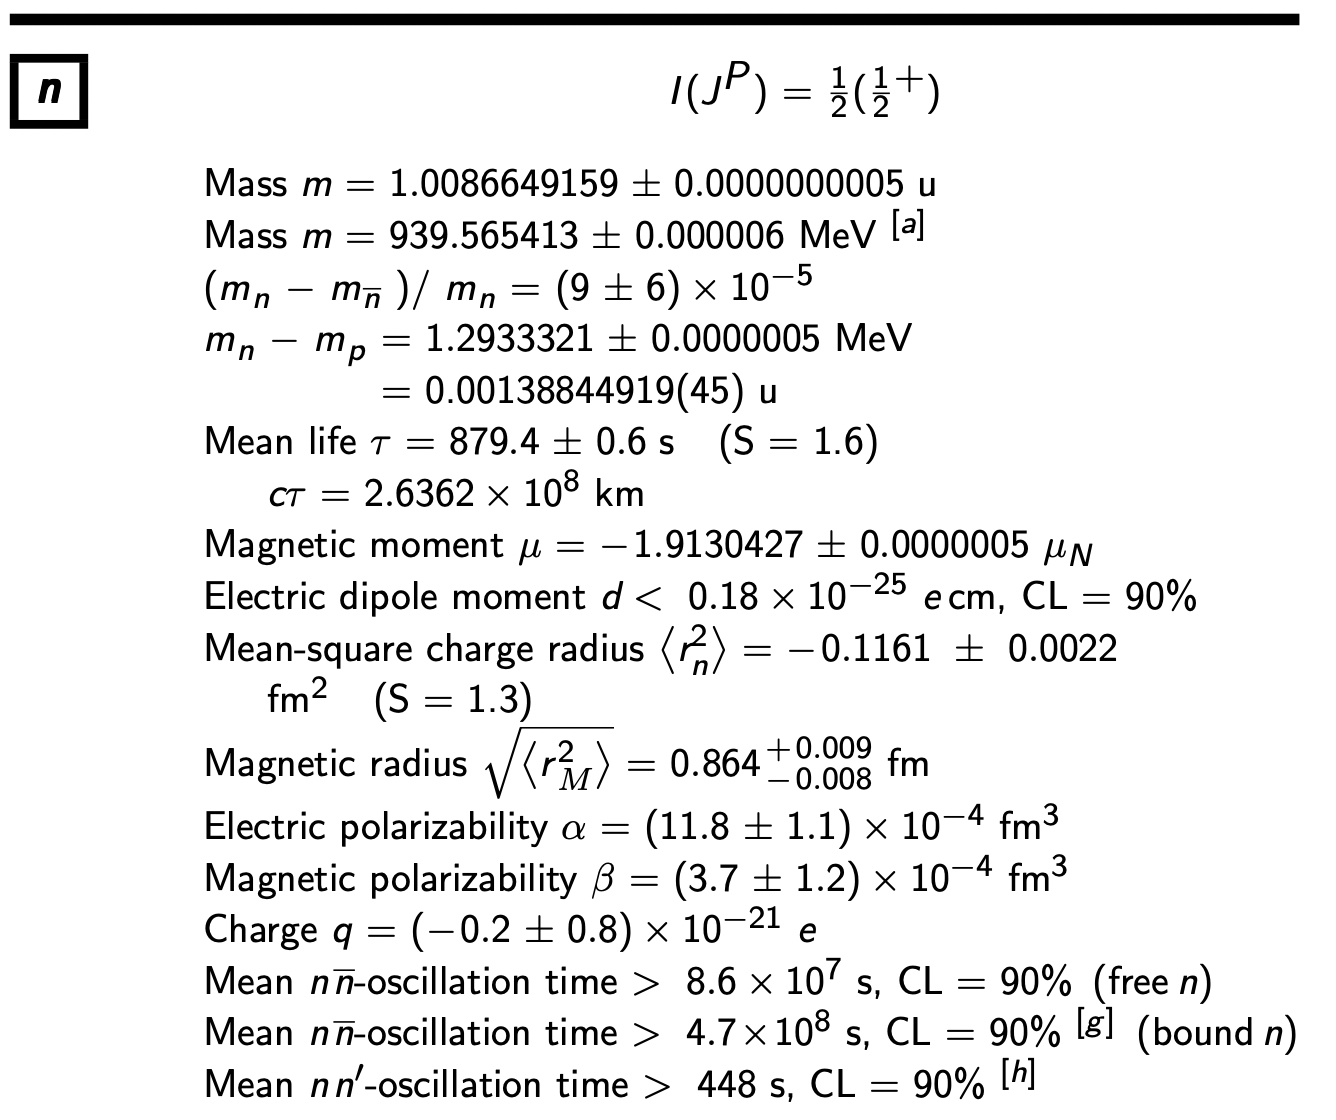
\includegraphics[width=0.8\textwidth]{PDG/neutron.png}
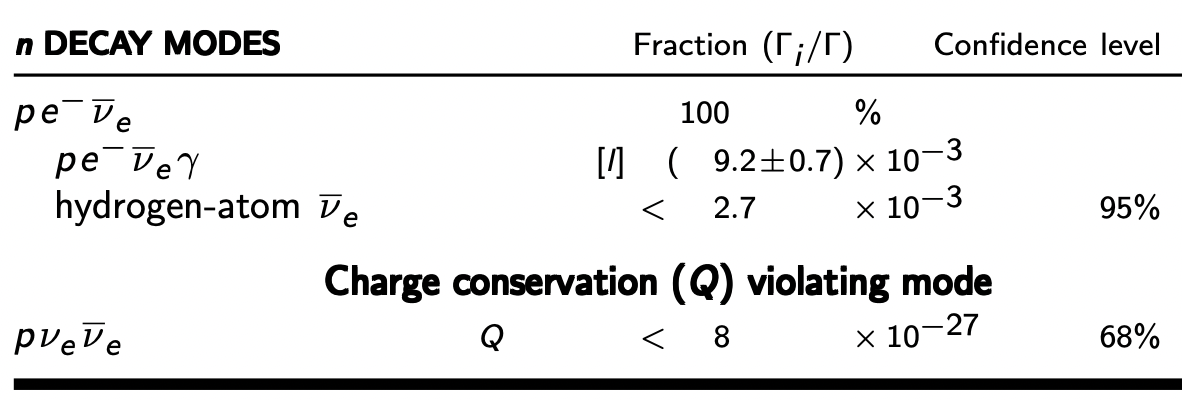
\includegraphics[width=0.8\textwidth]{PDG/neutron_DECAY_MODES.png}
%\clearpage
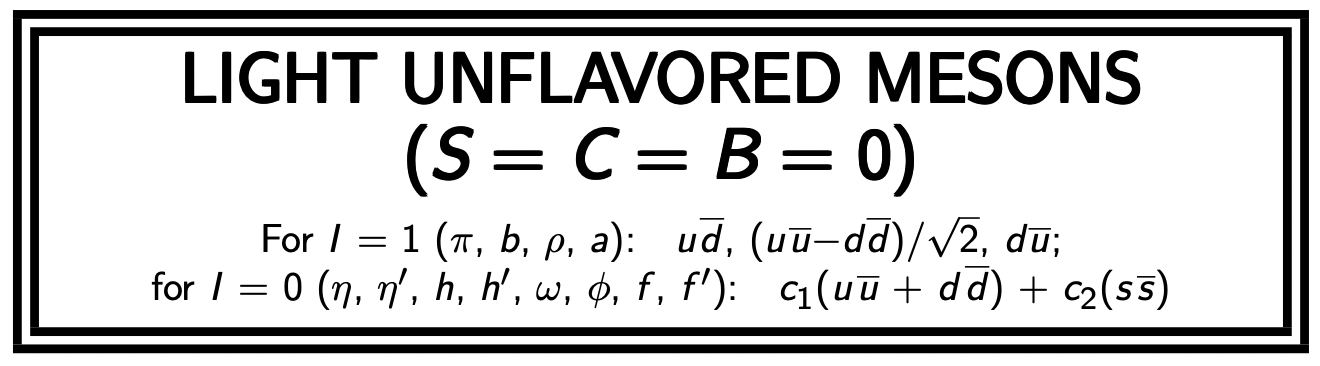
\includegraphics[width=0.8\textwidth]{PDG/LIGHT_UNFLAVOURED_MESONS.png}
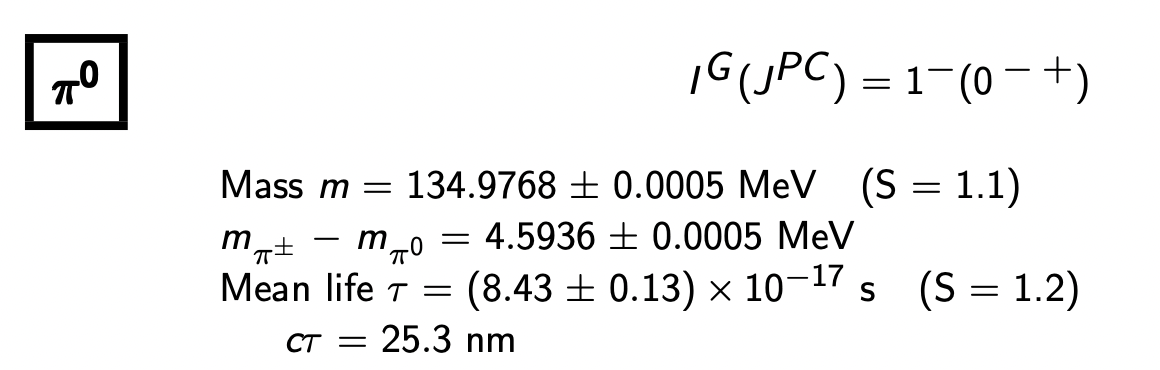
\includegraphics[width=0.8\textwidth]{PDG/PI_ZERO.png}
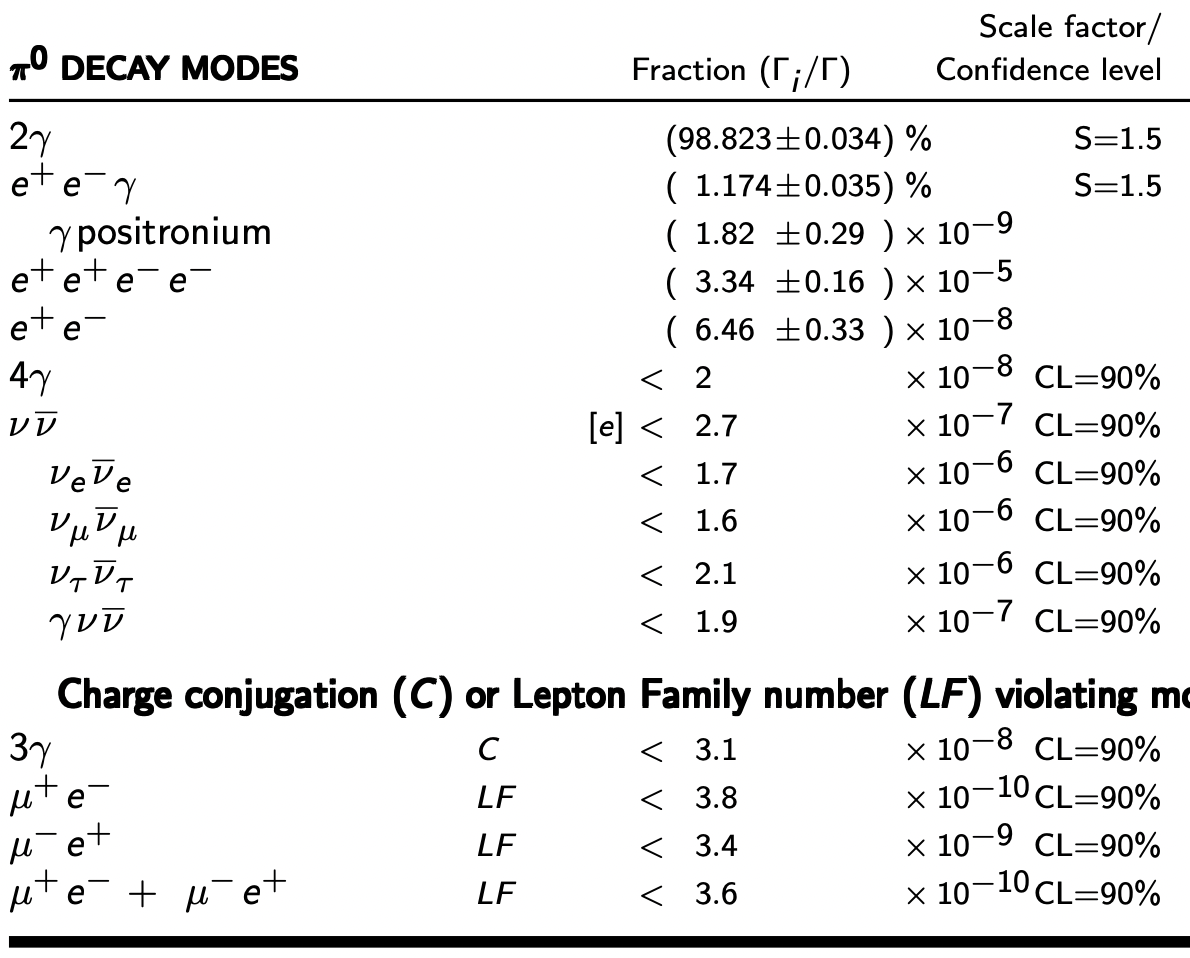
\includegraphics[width=0.8\textwidth]{PDG/PI_ZERO_DECAYS.png}
\clearpage
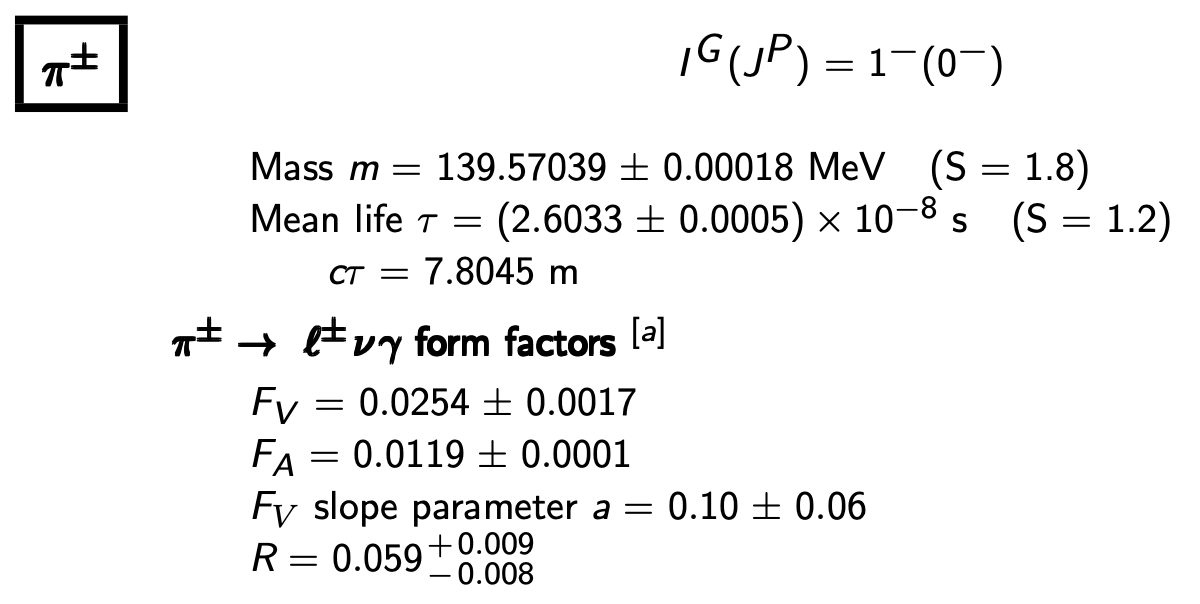
\includegraphics[width=0.8\textwidth]{PDG/PI_PLUS.png}
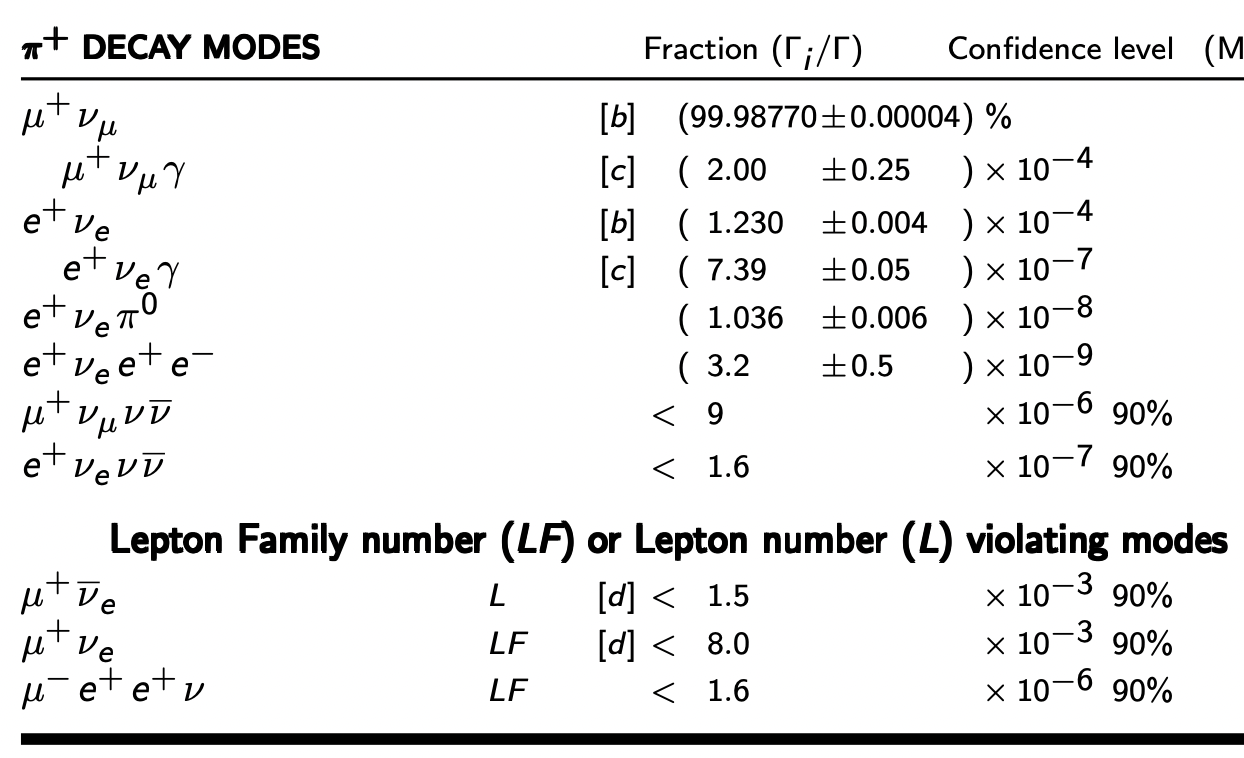
\includegraphics[width=0.8\textwidth]{PDG/PI_PLUS_DECAYS.png}
%\clearpage
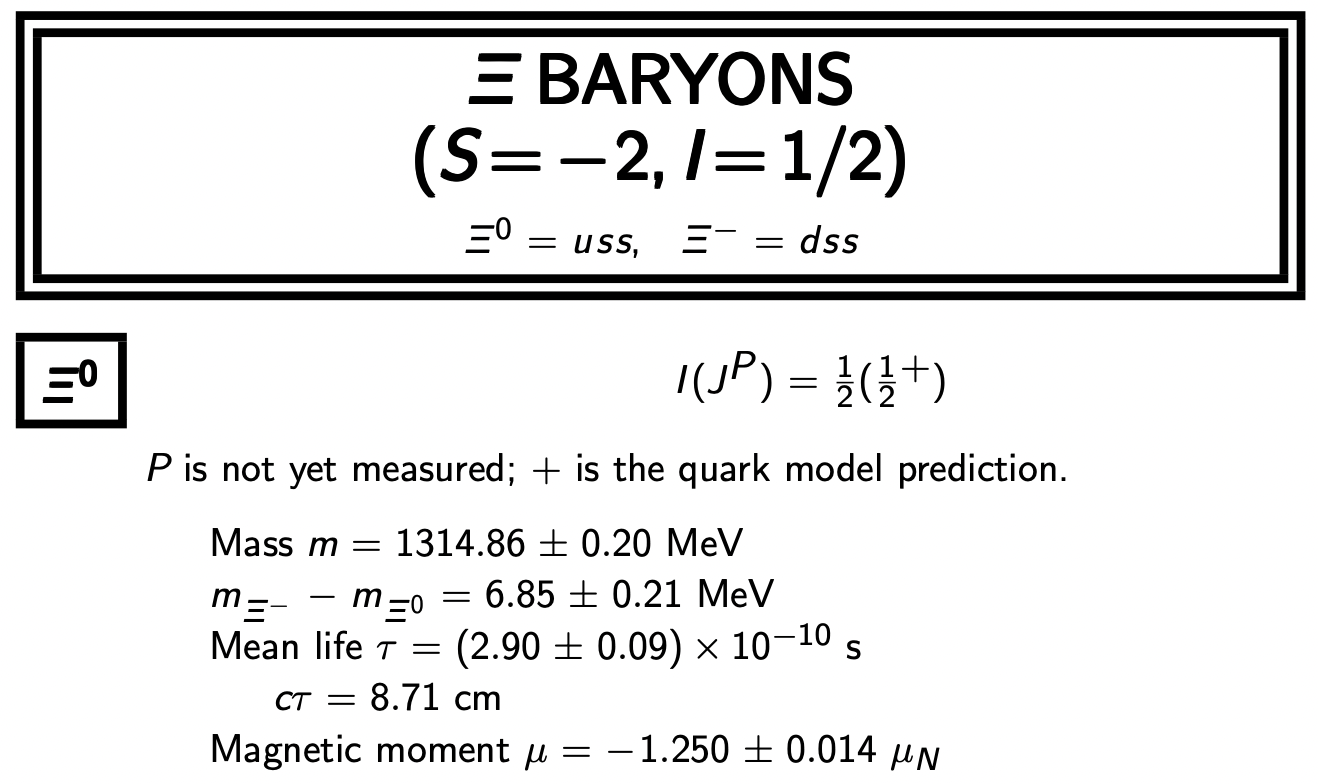
\includegraphics[width=0.8\textwidth]{PDG/XI_BARYONS.png}
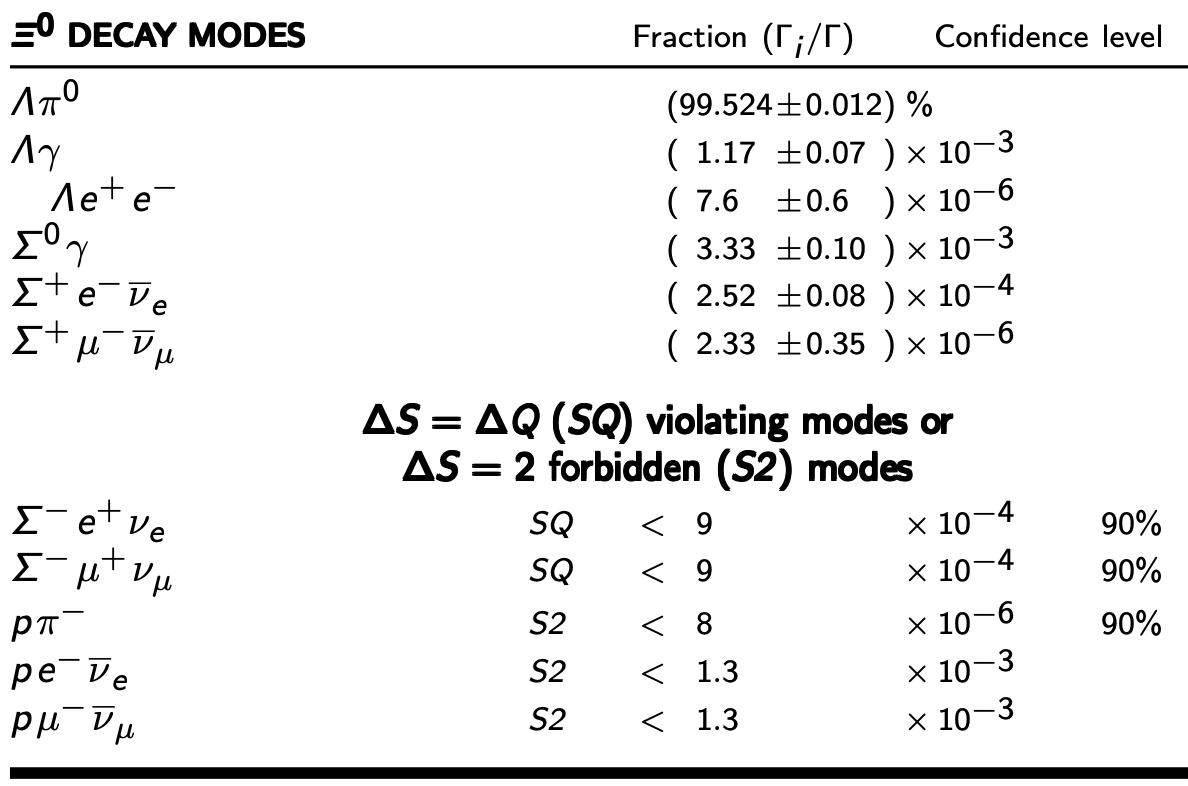
\includegraphics[width=0.8\textwidth]{PDG/XI_DECAY_MODES.png}
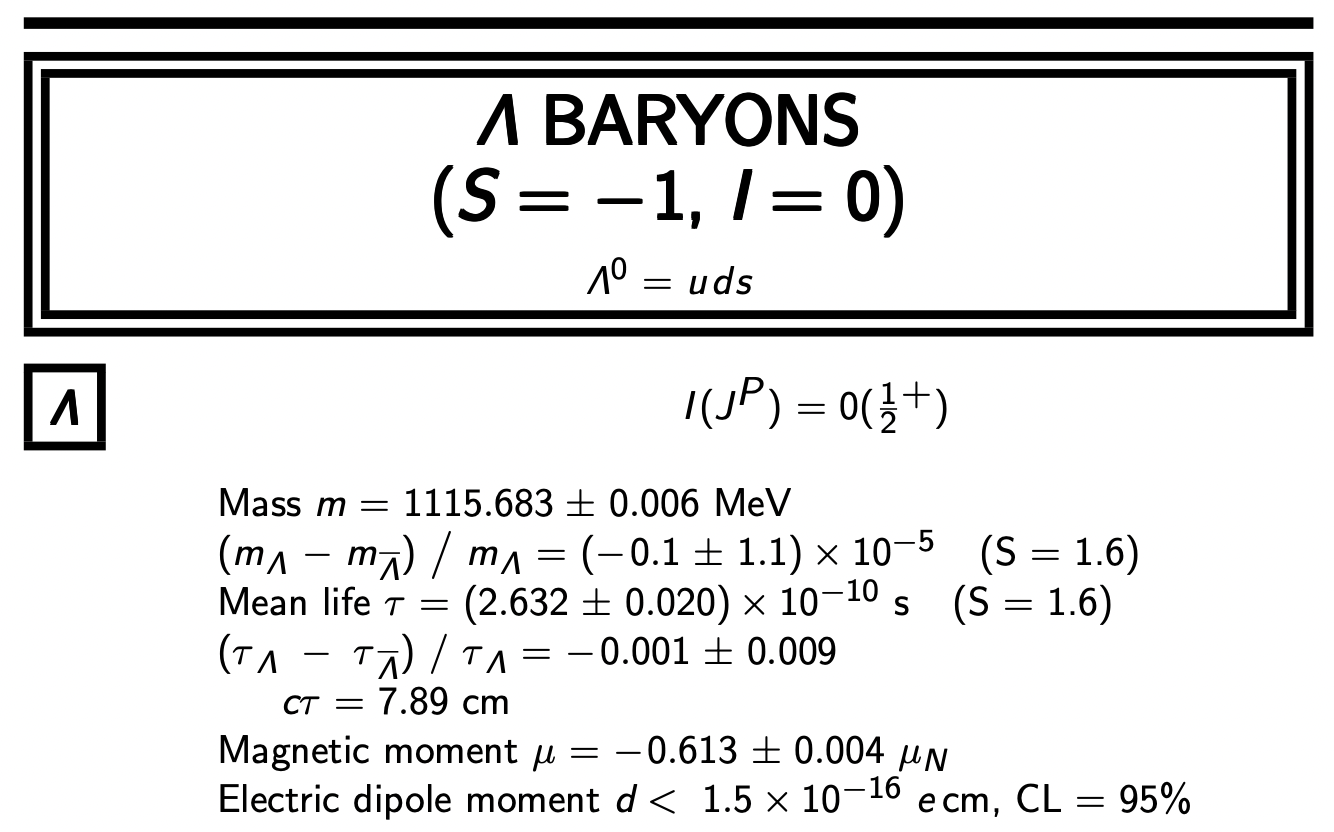
\includegraphics[width=0.8\textwidth]{PDG/LAMBDA_BARYONS.png}
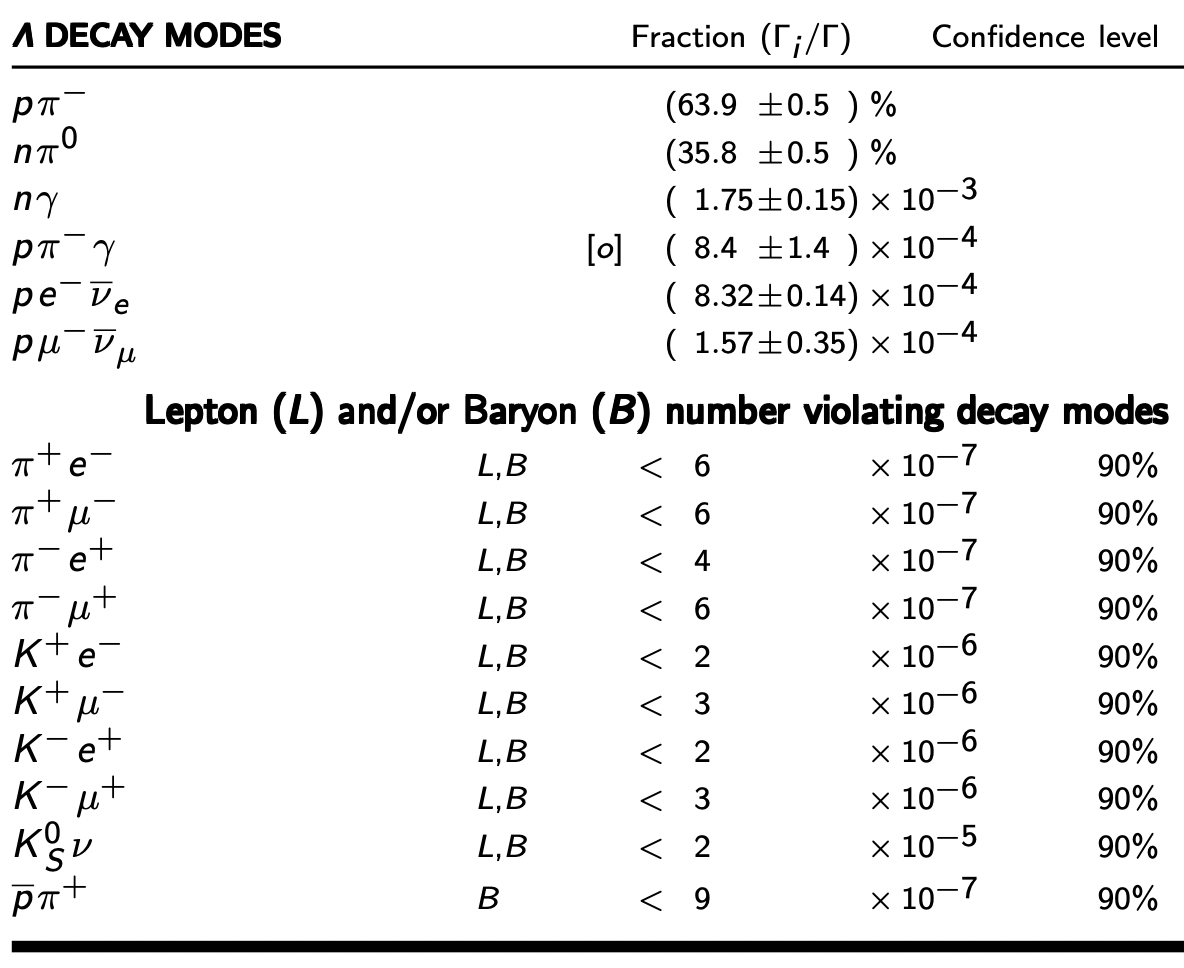
\includegraphics[width=0.8\textwidth]{PDG/LAMBDA_DECAY_MODES.png}
\end{center}